\chapter{Context: Clinical Measurements}
Cortical Bone is a highly organized, hard and lightweight tissue representing approximately 80\% of the skeletal mass in an human adult defined by an hierarchy of micro-structures. From a functional description, scaling down to nanometers its observed important structures for the cortical tissue such as haversian systems, osteons, lamellae, collagen fibres, fibrils, and elementary mineral constituents with water \cite{Parnell2008}. 

The standard description associated to a mechanical point of view is defining it as a two-phase composite material: a soft phase mainly of pores, containing organic fluid and soft tissues as cells, blood vessels, and a complex hard matrix phase with nerves distributed inside, being the matrix consisting mainly of hydroxyapatite and collagen. Porosity is distributed over various length scales, nevertheless only the two largest pores types: resorption cavities (with size of approx. $50-200 [\mu m]$ and haversian canal (size of approx. $50 [ \mu m ]$ contribute to the so-called mesoscale structure, thus the mechanical behavior of the cortical bone itself, hence the mesoscale porosity which is characteristic of the higher level of organization in bone. 

\begin{figure}[!h]
	\centering
	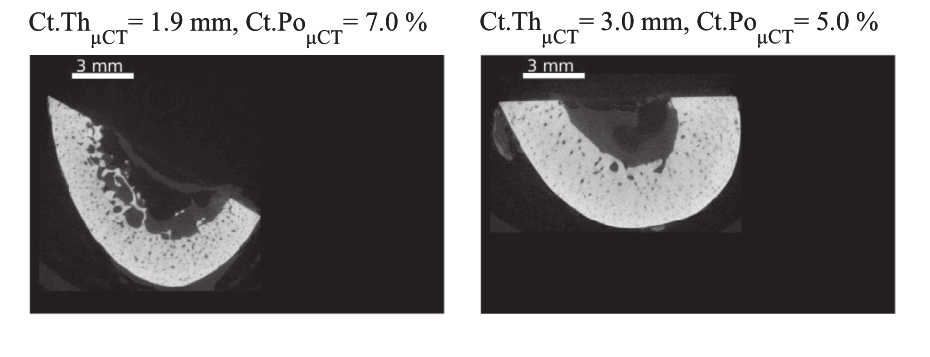
\includegraphics[width=0.9\textwidth]{images/ImgExt/CT-ImagesTwoCases.png}
	\caption{Real samples of $\mu$-CT transverse cross section images, with thickness $Ct.Th$ and porosity $Ct.Po$ labels, obtained from processing of the $\mu$-CT images itself \cite{Minonzio2018}. They define the standard clinical procedure for parameter measurement.}
	\label{muCT-Images}
\end{figure}

The study of such tissue gives us insights of various clinical parameters such as its microstructure, accumulated stress damage, collagen quality, bone turnover and others, necessary to diagnosis the status and quality of the bone itself, therefore to early diagnose of osteoporosis, a condition where less bone is added than taken away leading to skeletal fragility and increasing risk of fractures.

The early detection and prevention are important aspect of investigation. Dual X-ray Absorptiometry (DXA) provides the Bone Mineral Density (BMD) used to diagnose osteoporosis, defining the actual gold-standard.
As DXA provides non-volumetric measures of bone quality, for fidelity X-ray Quantitative Computed Tomography (QCT) is used to assess volumetric bone density, but is rather expensive with radiation costs involved. To overcome such aspects, new ultrasound techniques have been developed to assess relevant parameters of bone quality. It describes a lower cost, non-invasive nor radiative novel methodology that expects to reach the gold-standard predictions. But validations must be obtained and robustness research must be taken in consideration.

Under such setting, modelling and computational simulations of cortical tissues enables us to go further and test such new  procedures, validate under specific environments the possible outcomes and therefore assure the fidelity of results to clinical usage.


\section{Time-domain Modelling}

Sophisticated quantitative ultrasound (QUS) approaches under study \cite{Foiret2014} \cite{Minonzio2018}, are based on the axial transmission measurements which consist of guided waves recordings that propagate into and through the cortex in response to an ultrasonic excitation produced at the surface and then studying their response in the form of dispersion curves \footnote{From a physical perspective, its represented as the variation of wave number $k = 2 \pi f/c(f)$ as function of the frequency $f \in [0, 2]$ being $c(f)$ the phase velocity of the mode.}, i.e., by means of the \textit{Lamb}-waves nonlinear equations \cite{Rhee2007}.
Wave-guide characteristics such as thickness and porosity can then be deduced from the dispersion curves by finding the best fitting of theoretical wave-guide model to experimental data after a signal processing step. Such procedure define in particular the inverse problem under consideration.

In this section, it is described the experimental procedure used to study two bone mechanical properties by means of a ultrasound transducer.
It is also given a brief explanation of the setting involved in the clinical procedure and the assumptions being done to model the recorded signal then processed by a spectrum technique. 

\subsection{Experimental Procedure}
The bone sample studies are subjected to the transmission of the wave-guide, i.e., a wave propagated from the external surface generated by a transducer device. 
Explicitly such force can be considered in the form:
\begin{equation*}
    \mathbf{F}(\mathbf{x},t) = A e^{-\frac{(t-t_0)^2}{2\sigma_0^2}} cos(2 \pi \tau_0 (t-t_0)) \text{ on } \Gamma_N
\end{equation*}
where $A > 0$ denotes an amplitude, $t_0 > 0$ a central time, $\tau_0$ some period, $\sigma_0>0$ a fixed variance and $\Gamma_N$ surface boundaries where the force is applied.

Even though the shape of long segments of cortical bone is not uniform with respect to thickness nor in its surface, because of the device shape and size, it can be considered that such local spatial variations in the geometry are minimum and moreover can be neglected \cite{Foiret2014}. As the transducer device captures the wave-guide over the long axis of bone, the propagation effects given on the non-axial (or anti-plane) of the wave are assumed to not add more relevant features in such a way that the natural 3-dimensional cylindrical-like shape of the bone can be simplified without affecting the overall behavior of interest to a 2-dimensional plate shape domain modelling the coronal cut plane of propagation. \\

For such a 2-dimensional wave-guide model, the propagation is studied by means of the homogenization technique in elastic and viscoelastic behaviors. Such a homogenization procedure results necessary since the size of microstructure generates restrictive computational costs, and moreover the ability of such theory to model the microstructure observed for example in (\ref{muCT-Images}), i.e., containing the porosity level implicitly in the elastic coefficients obtained by means of two-scale asymptotic framework.  Schematically, figure (\ref{SchematicProp&Hom}) describes the experimental and the assumptions on the cortical tissue. \\

\begin{figure}[!h]
	\centering
	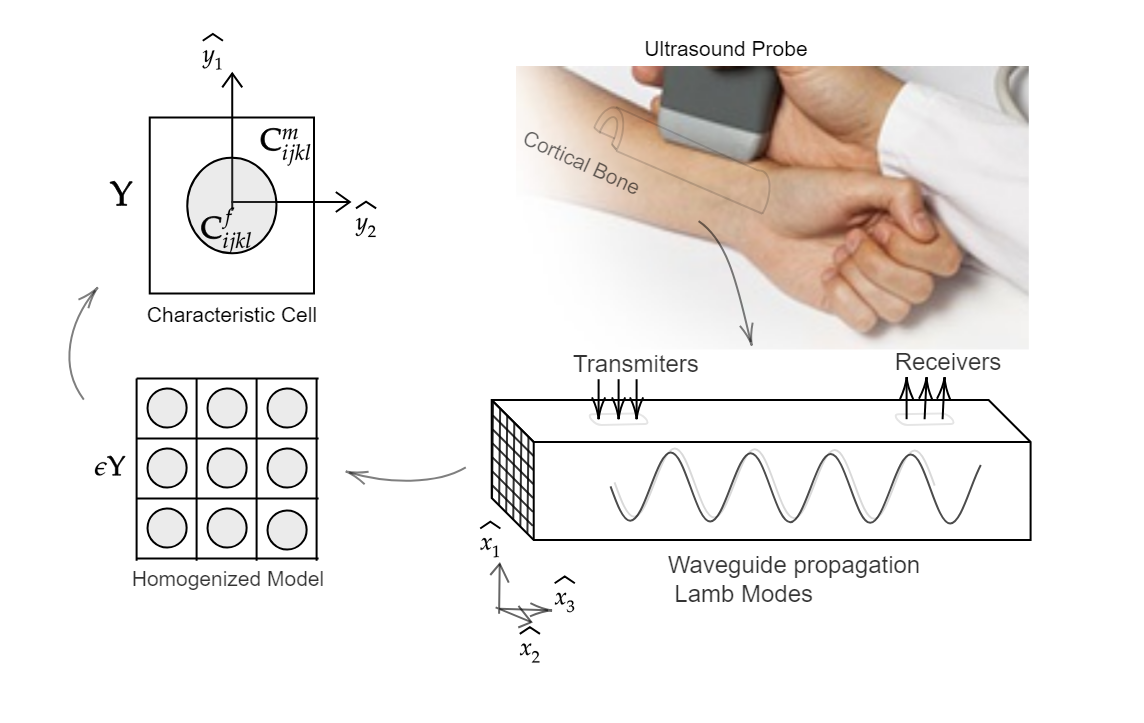
\includegraphics[width=0.8\textwidth]{images/ImgExt/SchematicPropagation.png}
	\caption{Schematic Procedure: from the experimental device to the homogenize idealization of the cortical bone.}
	\label{SchematicProp&Hom}
\end{figure} 

The important aspect of the transducer is the linear element array which contains several emitters and receiver. It is modeled the experimental setting of the transducer applied on patients as an elastodynamic model defined on the cortical bone, moreover it is neglected the effects at the interface with the skin. The excitation generated at the surface by the transducer is produced by different force-sources acting independently, more explicitly by an array of 8-source forces generating each one a wave-propagation, enabling the posterior recordings at the receiver locations. Nevertheless, by assuming symmetric and regular domains, each wave-propagation has equal mechanical effects by the translation invariance properties of the elastic wave which enables us to reduce time-costs for numerical implementations. 

\subsection{Signal Processing}
Each cycle of measurements consists of a sequential excitation of $N^E > 0$ number of emitters located at boundaries $\Gamma_{e_i}$ for each $i \in \{1,\dots, N^E\}$ where the device recordings take place. By denoting $N^R>0, N^T>0$ the number of receivers and number of discretization steps respectively, the device yields $N^T \times N^R$ arrays from each emitter.

Such signal generated by the excitation of each emitter $m \in \{1,\dots, N^E\}$ denoted by $s_m(t, \mathbf{x})$ at fixed time $t$ and receptor position $\mathbf{x}$ is \textit{Fourier} transformed to the frequency domain denoting such signal by $S_m(f, \mathbf{x})$ at fixed $f \in \mathbb{R}_+$, associated to a frequency discretization bandwidth of $N^F > 0$ steps.

The spectral description of the propagated wavefront which allows a comparison regarding the \textit{Lamb}-waves \footnote{Several studies consider the usage of this kind of curves, as ones mainly used to describe the material destruction and mechanical behavior, and moreover in a non-invasive form \cite{Rhee2007}.} is obtained from a Singular Vector Decomposition (SVD) over the signal $(S_n(t, \mathbf{x})_{n \in [N^E]}$.
Explicitly, the signal array is decomposed in the form:
\begin{equation*}
    S_n = U_n \sigma_n D_n, \quad n \in \{1,\dots, N^E\}
\end{equation*}
being each array $U_n \in \mathcal{M}_{N^F\times N^R}, \sigma_n \in \mathcal{M}_{N^R\times N^R}, D_n \in \mathcal{M}_{N^R \times N^R}$ associated to the frequency and receptor discretization arrays.
The singular value bases $(U_n)_n$ are then used to define a function for frequency-wavenumber pairs $(f,k) \in \mathbb{R}_+ \times \mathbb{R}$ in the form:
\begin{equation*}
    L_N(f, k) = \sum_{n = 1}^{N} \big \vert \langle U_n(f,\mathbf{x}) \, \vert\, e^{ik\mathbf{x}} \rangle \big \vert^2
\end{equation*}
being $0 < N \leq N^E $ the intensity mode number, allowing the description of wave-modes recorded on the $(f,k)$ space by applying the plane wave projector operator over the bases $U_n$. In particular, since the wave-number $k$ is dependent on the material properties as $(Th, Po)$ then it arises the experimentally obtained wave-modes described by $L_M(f,k(Po, Th))$ enabling comparison to the \textit{Lamb}-wave material curves.

 Experimentally, figure (\ref{RealLM-Images}) shows two particular cases of \textit{Lamb}-waves recordings, each describing the symmetric and anti-symmetric modes characteristic of each material.

\begin{figure}[!h]
	\centering
	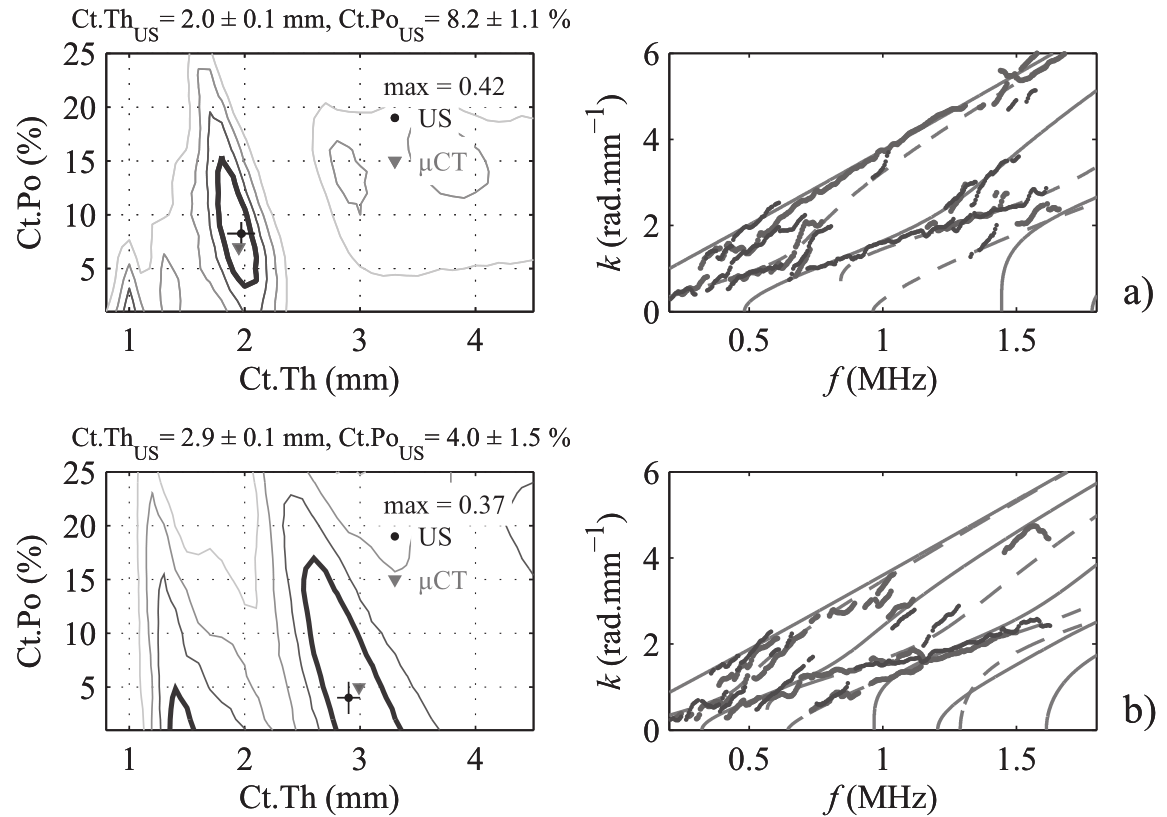
\includegraphics[width=0.9\textwidth]{images/ImgExt/FKDiagramTwoCases.png}
	\caption{On the left side, objective functional of (\ref{muCT-Images} associated to the minimization problem (\ref{Min-Problem}) in $(Po, Th)$ parameters with the best acquisition are shown by the circle and triangles. On the right side, the experimental dispersion curves (dots) with the guided modes (continuous and dashed lines) describing the \textit{Lamb} reference curves. The obtained values by $\mu$-CT and ultrasound technique are indicated in the $(Th, Po)$ plane with black circles and gray dots respectively. While the $L_4(f,k)$ dispersion curves are described by dots fitting the reference \textit{Lamb}-curves \cite{Minonzio2018}.}
	\label{RealLM-Images}
\end{figure}

Thus, the parameter recuperation (or inverse problem) from recorded signals is defined by the optimization problem:
\begin{equation}
    (Po^*, Th^*) = \underset{(Po, Th) \in \mathcal{A}}{\text{argmax}} \int\limits_{f_{min}}^{f_{max}} \frac{1}{N} \sum_{m=1}^{M} L_N(f, k_m(Po, Th)) \,df 
    \label{Min-Problem}
\end{equation}

being $M>0$ the number of modes and $\mathcal{A}$ the space of porosity $\times$ thickness pairs. Therefore, the formulation is re-expressed as the recuperation of $(Th.^*, Po.^*)$, two relevant biomedical parameters describing the quality of cortical bone.

An important aspect of such \textit{Lamb} curves is the fact that implicitly contain the overall mechanical behavior of the elastodynamic model, so that define a useful tool for validation and comparison of numerical simulation with respect to real data  \cite{Rhee2007}. Over such a domain it is considered their behaviour of linear elastic type, defined by a displacement $u(\mathbf{x},t)$ with constitutive equation following \textit{Hookes} law and forces $\mathbf{F}(t)$ applied at a section of the surface.

\section{Main assumptions and Multiscale Modelling}

Computational modelling of biological tissues (in particular of bone) is a complex multiscale problem, since there are multiple physical phenomena interacting at various scales. Moreover, in a bast majority of clinical applications the material is viewed as continuum, thus it is important to contribute with a mathematical model and numerical procedures to characterize non-trivial properties arising from the microscopic geometrical structures affecting the overall behavior in terms of effective compressibility (or viscosity) or elasticity. 

Formally it is considered the following:
Let a bounded domain $\Omega \subset \mathbb{R}^d$ ($d = 2,3$) represent the composed material under study, modeled by an elastic matrix with several inclusion defining the so-called mesoscale being described mechanically by an elastic of cylindrical shape periodically distributed.
For the sake of the experimental setting under consideration, the exterior boundary $\partial \Omega$ is decomposed as
\begin{equation*}
	\partial \Omega = \Gamma_D \dot\cup \Gamma_N
\end{equation*}
denoting $\Gamma_D, \Gamma_N$ the Dirichlet and Neumann part of the exterior boundary respectively.

Furthermore, let the small parameter $0 < \epsilon \ll 1$ denote the aspect ratio between the macroscopic variable $\mathbf{x} \in \Omega$ and the microscopic one $\mathbf{y}$ in the form: $\mathbf{y} = \frac{\mathbf{x}}{\epsilon}$ being $\mathbf{y} \in \mathbf{Y}$ and $\mathbf{Y} = (0,1)^d$ the cell structure. In this configuration, the unitary cell $\mathbf{Y}$, can be decomposed as
\begin{equation*}
	\mathbf{Y} = \mathbf{Y}_m \cup \Gamma \cup \mathbf{Y}_p 
\end{equation*}
where $\mathbf{Y}_m$ and $\mathbf{Y}_p$ are defined as the domains occupied by the matrix and porous part respectively, and $\Gamma$ denotes the interface between them\footnote{This model is inspired in the development of the Homogenization of the elastic operator in a porous media proposed on \cite{christensen1982theory}. Nevertheless, this kind of configurations are typical in the two-scale homogenization literature \cite{panasenko2005multi-scale}, \cite{Boughammoura2013} to mention updated references.}.

Such a cell is assumed to be periodically distributed along the material, defining its highly oscillatory structure, suitable to use the the Homogenization framework. It is considered the composite material of study with elastic properties having oscillation rate $\epsilon$, represented in the domain decomposition:
\begin{equation*}
	\overline{\Omega} = (\overline{\Omega}\setminus \Omega_1^{\epsilon}) \cup \overline{\Omega}^{\epsilon}_1
\end{equation*}
defined by:
\begin{equation*}
    \overline{\Omega}^{\epsilon}_1 = \bigcup_{\mathbf{x} \in \mathbf{T}_{\epsilon}} \epsilon ( \mathbf{x} + \mathbf{Y} )
\end{equation*}
being the tessellation $\mathbf{T}_{\epsilon}$ the subset in $\mathbb{Z}^d$ of all points satisfying the conditions
\begin{equation*}
    \epsilon (\mathbf{x} + \mathbf{Y}) \subset \Omega, \quad \rho(\epsilon(\mathbf{x}+\mathbf{Y}), \partial \Omega) \geq \epsilon
\end{equation*}

Let us note in particular that for fixed $\epsilon >0$ and all $\mathbf{x} \in \Omega$ there is a unique decomposition $\mathbf{x}/\epsilon = \mathbf{x}_{\mathbf{T}_{\epsilon}(\mathbf{x})} + \mathbf{y}$ where $\mathbf{x}_{\mathbf{T}_{\epsilon}(\mathbf{x})}$ denotes the element in $\Omega$ of the tessellation.

The above considerations allow us to define finally the material coefficients as second order rank tensors for component $i,j,k,l \in \{1,\dots, d\}$ in the form:
\begin{equation*}
    C_{ijll}(\frac{\mathbf{x}}{\epsilon}) = C_{ijkl}(\mathbf{y}) \quad \text{for } \frac{\mathbf{x}}{\epsilon} = \mathbf{x}_{\mathbf{T}_{\epsilon}(\mathbf{x})} + \mathbf{y}, \, \mathbf{x} \in \Omega_1^{\epsilon}
\end{equation*}
and being $C_{ijkl}(\frac{\mathbf{x}}{\epsilon}) = 0$ if $\mathbf{x} \in \overline{\Omega} \setminus \Omega_1^{\epsilon}$.

\begin{figure}[!h]
	\centering
	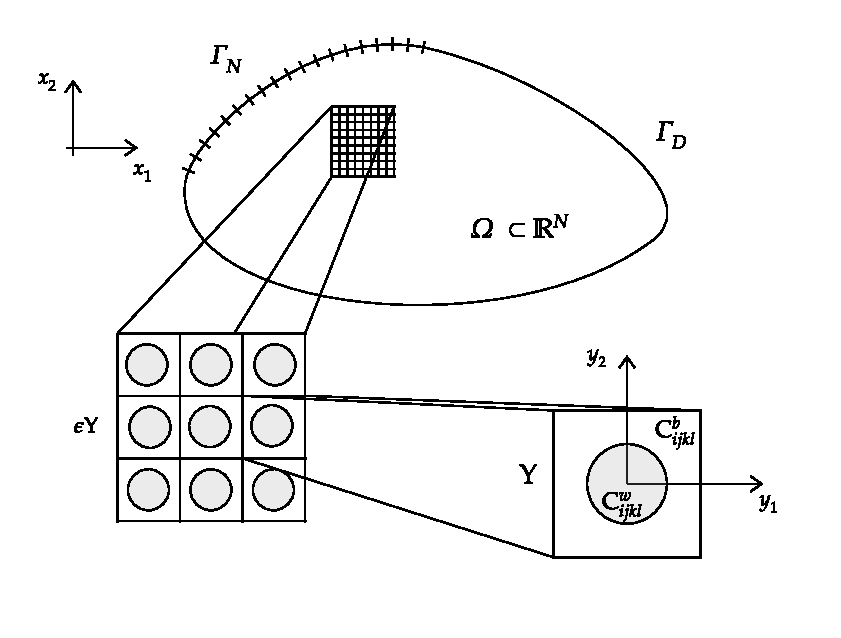
\includegraphics[width=0.8\textwidth]{images/HomSchemes/HomBasicScheme.pdf}
	\caption{Two-Scale homogenization assumption for the microstructure, defining it as a highly oscillatory composite material, periodically distributed along the the anti-plane symmetric over the long-axis of bone.}
	\label{HomBasicScheme}
\end{figure}

\begin{rem}
The material is assumed to be confined within the inclusion as a elastic (emulating a mechanical behavior of blood mixture mainly made of saturated static fluid) with volume $\epsilon^d \vert \mathbf{Y}_p \vert$ embedded in a elastic material (modeled mainly of hydroxipatite and collagen) filling a unit cell of volume $\epsilon^d \vert \mathbf{Y} \vert$.
It is defined, after scaling, the porosity associated to the material as the fraction of volume occupied by the gas in the unitary cell, i.e., 
\begin{equation*}
\phi = \frac{\vert \mathbf{Y}_p \vert}{\vert \mathbf{Y} \vert} = \vert \mathbf{Y}_p \vert
\end{equation*}
which will define the material coefficients dependent of such parameters.
\end{rem}

Thus, denoting the observed displacement $u(\mathbf{x},t) \in \mathbf{H}^1(\Omega)$ with behaviour of linear elastic type subjected to surface forces $\mathbf{F}(t) \in L^2 (0, T)$, the material is assumed to behave following the system of partial differential equations (PDE's) in the form:
\begin{equation*}
    \left \{
    \begin{aligned}
        \rho (\frac{\mathbf{x}}{\epsilon}) \partial_{tt} u^{\epsilon}(\mathbf{x},t) - \nabla \cdot \sigma (u^{\epsilon}(\mathbf{x},t)) & = \mathbf{0}, \text{ in } (0,T)\times \Omega \\
        \sigma(u^{\epsilon}(\mathbf{x},t))_{ij} = \mathbf{C}_{ijkl}(\frac{\mathbf{x}}{\epsilon}) \mathbf{e}_{kl}(u^{\epsilon}(\mathbf{x},t)) & \text{ in } (0,T)\times \Omega \\
        u^{\epsilon}(\mathbf{x},t) = \mathbf{0} & \text{ on } (0,T)\times \Gamma_D\\
        \sigma(u^{\epsilon}(\mathbf{x},t)) \cdot n = \mathbf{F}(t) & \text{ on } (0,T)\times \Gamma_N
    \end{aligned}
    \right .
\end{equation*}

where $\mathbf{C}(\mathbf{x})$ denotes the elasticity tensor, $\rho(\mathbf{x})$ the material density and $\mathbf{e}(u(\mathbf{x},t)) = \frac{1}{2}\big( \nabla u(\mathbf{x},t) + \nabla u(\mathbf{x},t)^{T}\big)$ the symmetric gradient, each at position $\mathbf{x}$ and time $t \in (0,T)$. As shown, the clear dependency on the $\epsilon$ scale requires a more complex framework to successfully implement a feasible numerical model, which will be the two-scale asymptotic theory, developed in the next chapter.


